\lstinputlisting[language=bash,basicstyle=\small]{python_codes/fieldstone_12/keywords}

\begin{center}
Code at \url{https://github.com/cedrict/fieldstone/tree/master/python_codes/fieldstone_12}
\end{center}

\par\noindent\rule{\textwidth}{0.4pt}
%%%%%%%%%%%%%%%%%%%%%%%%%%%%%%%%%%%%%%%%%%%%%%%%%%%%%%%%%%%%%%%%%%%%%%%%%%%%%%%%%%%%%%%%%%%%%%


We start from the analytical benchmark of Section \ref{mms1} and we use $Q_1 \times P_0$
elements with a penalty formulation. 
We have seen in stone $\# 1$ how to recover the elemental pressure as a postprocessing step. 
However, the discontinous nature of the pressure field (and the presence of a
parasitic checkerboard mode) can be problematic for many reasons 
(pressure enters the rheology, equation of state, plotting, ...). 
We then wish to project the elemental pressure onto the nodes of the mesh while at the same 
time filtering the checkerboard mode out. 

Terminology: in general, when a discontinuous elemental pressure is used in a stone, 
it is called $p$ while its projection onto the nodes is coined $q$. 
In this case we compute several nodal pressures as explained in Section~\ref{psmoothing}:

\begin{itemize}
%...........
\item $q_1$: smoothed pressure obtained with the  center-to-node approach (scheme 1)

\item $q_2$: the nodal pressure obtained by smoothing the elemental pressure using element areas (scheme 2)

\item $q_3$: the nodal pressure obtained by smoothing the elemental p using triangle areas (scheme 3)

\item $q_4$: smoothed pressure obtained with the center-to-node approach with inverse element area weighing.

\item $q_5$: is not computed because same as 6.

\item $q_6$: consistent pressure recovery through FE (scheme 5 \& 6)

\item $q_7$: consistent pressure recovery with lumped mass matrix. 

\item $q_8$: bilinear interpolation. 

\end{itemize}

Since the setups showcase Dirichlet boundary conditions on all four sides, 
the pressure solution is normalised so that $\int p dV =0 $.

\begin{remark}
Nodes on edges and corners may need special treatment as documented in Sani et al \cite{sagl81a} or
Lee et al (1979) \cite{legs79} which is not done here.  
\end{remark}

\begin{remark}
Lee et al (1979) \cite{legs79} discuss two different ways to compute the lumped mass matrix. 
\end{remark}

\begin{remark}
Nodes on the boundary showcase the largest errors. Maybe then use CBF instead for these?
\end{remark}

\begin{remark}
In the same folder there is a fortran90 version of the consistent recovery algorithm.
\end{remark}


I have created a simple checkerboard filter. Let $\phi=\pm 1$ denote this field.
The filter is applied as follows:
\[
p_{filtered} = p - \left( \frac{1}{|\Omega|} \iint_\Omega p \phi dV \right) \phi
\]
It is in fact a a projection. If $p=\alpha \phi$  where $\alpha$ is a scalar, then 
it is trivial to show that $p_{filtered} =0$.
Likewise, if $p=constant$ then $p_{filtered}=p$.
This idea is probably to be found in the relevant publications of Section~\ref{psmoothing}
in some form or shape. 

There is much more work to be done on this topic/stone!

\newpage
%...............................................
%...............................................
\paragraph{Regular mesh made of square elements}

We compute the error convergence for $p$, $q_i$ $(i=1,...8)$:
\begin{center}
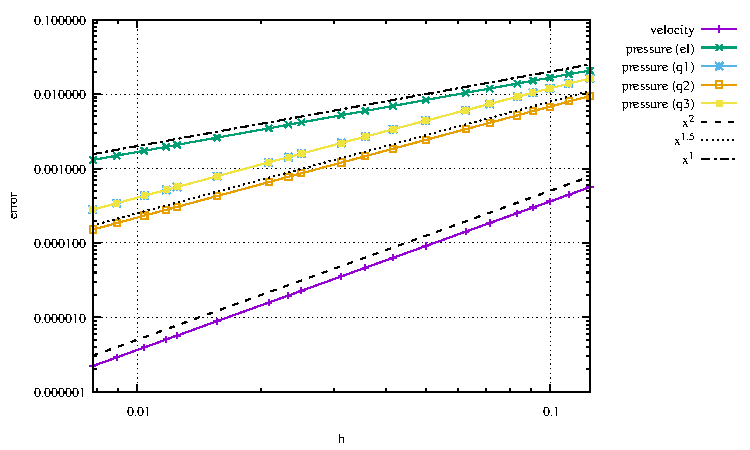
\includegraphics[width=10cm]{python_codes/fieldstone_12/results/reg/errors}
\end{center}
The elemental pressure error converges like $h^1$, $q_{1-7}$ converge like $h^{1.5}$ and 
$q^8$ converges like $h^2$.


\begin{center}
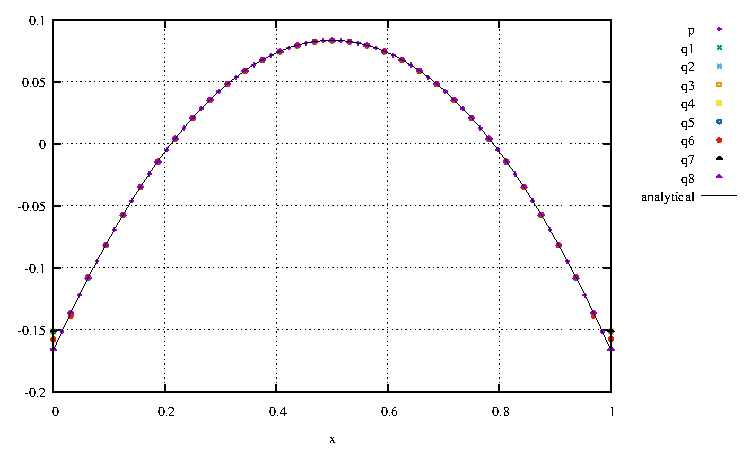
\includegraphics[width=5cm]{python_codes/fieldstone_12/results/reg/pressure}
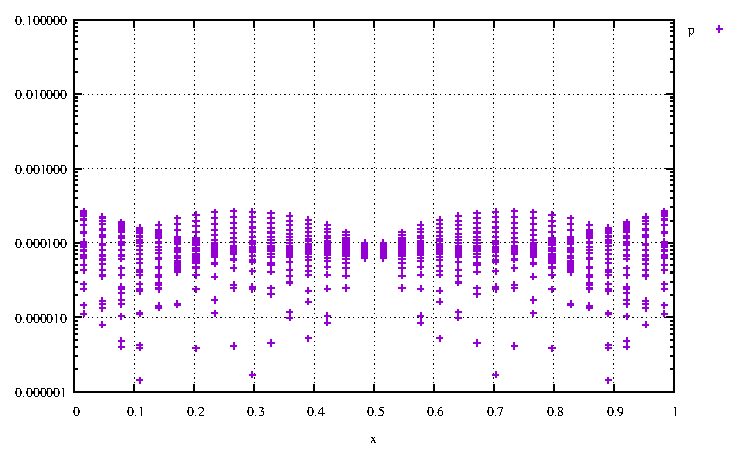
\includegraphics[width=5cm]{python_codes/fieldstone_12/results/reg/p_error}
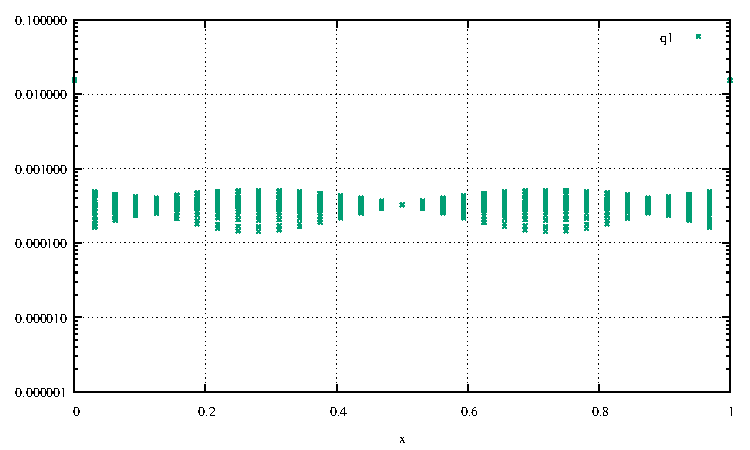
\includegraphics[width=5cm]{python_codes/fieldstone_12/results/reg/q1_error}\\
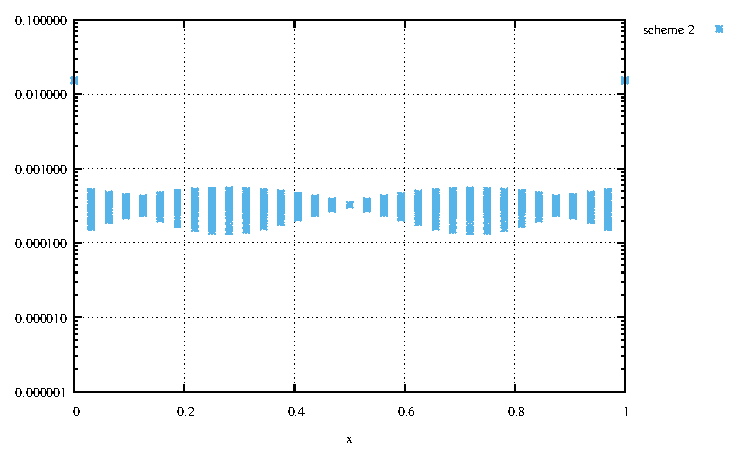
\includegraphics[width=5cm]{python_codes/fieldstone_12/results/reg/q2_error}
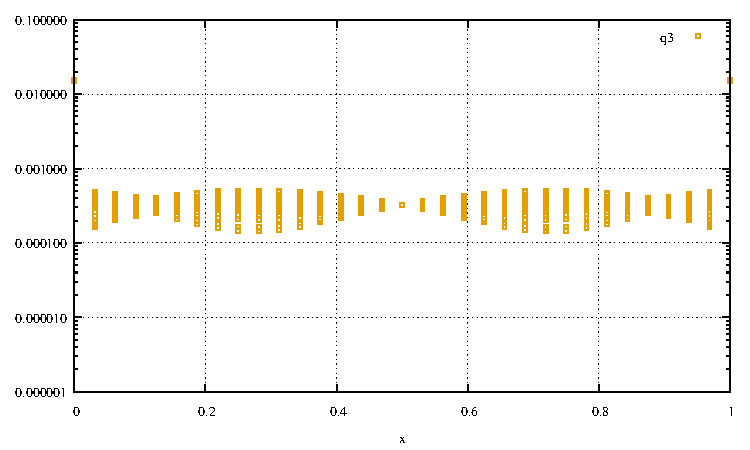
\includegraphics[width=5cm]{python_codes/fieldstone_12/results/reg/q3_error}
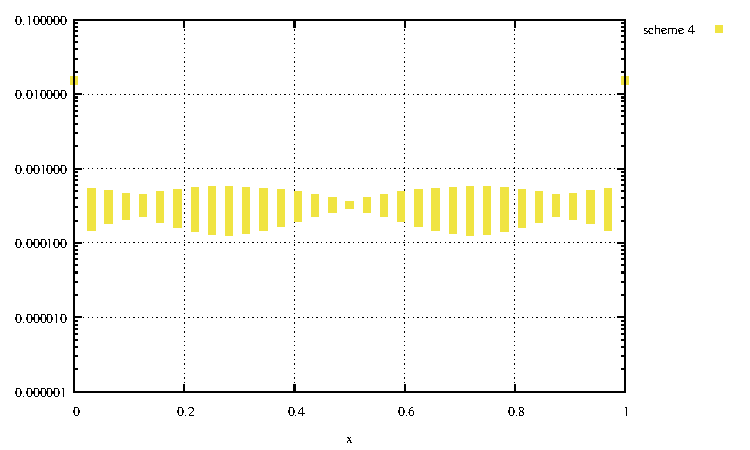
\includegraphics[width=5cm]{python_codes/fieldstone_12/results/reg/q4_error}\\
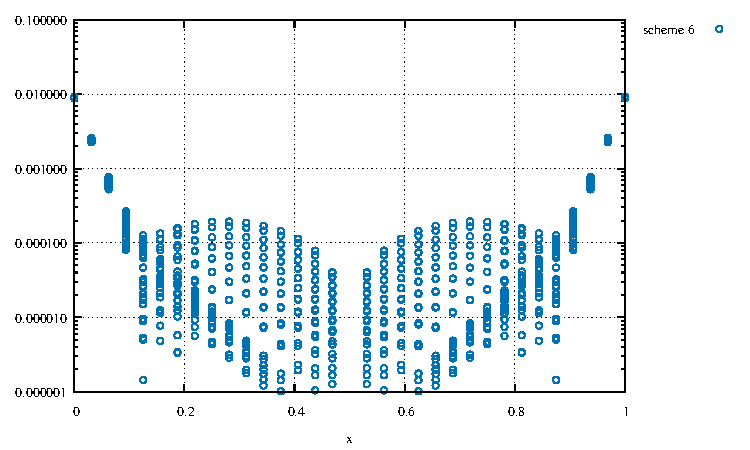
\includegraphics[width=5cm]{python_codes/fieldstone_12/results/reg/q6_error}
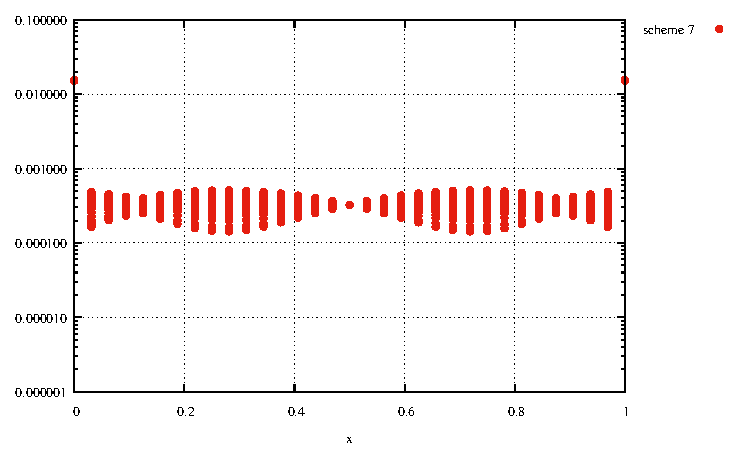
\includegraphics[width=5cm]{python_codes/fieldstone_12/results/reg/q7_error}
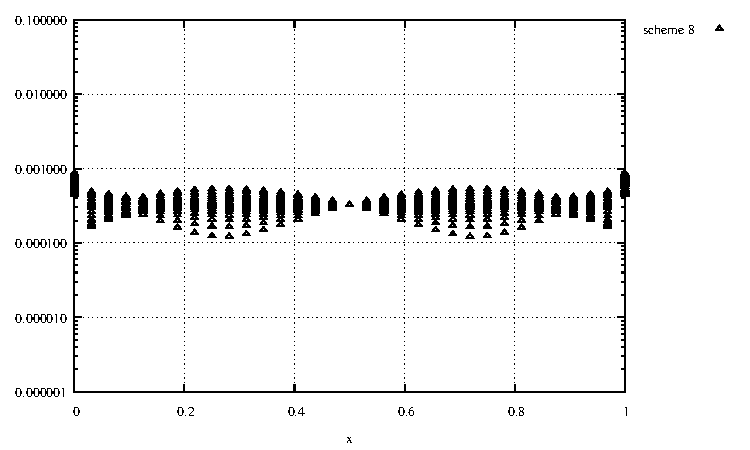
\includegraphics[width=5cm]{python_codes/fieldstone_12/results/reg/q8_error}\\
{\captionfont Left: pressure fields as a function of the $x$-coordinate. 
Right: absolute error with regards to the analytical solution. All on 32x32 mesh.}
\end{center}

It is worth noticing that the checkerboard is (visually) not present:
\begin{center}
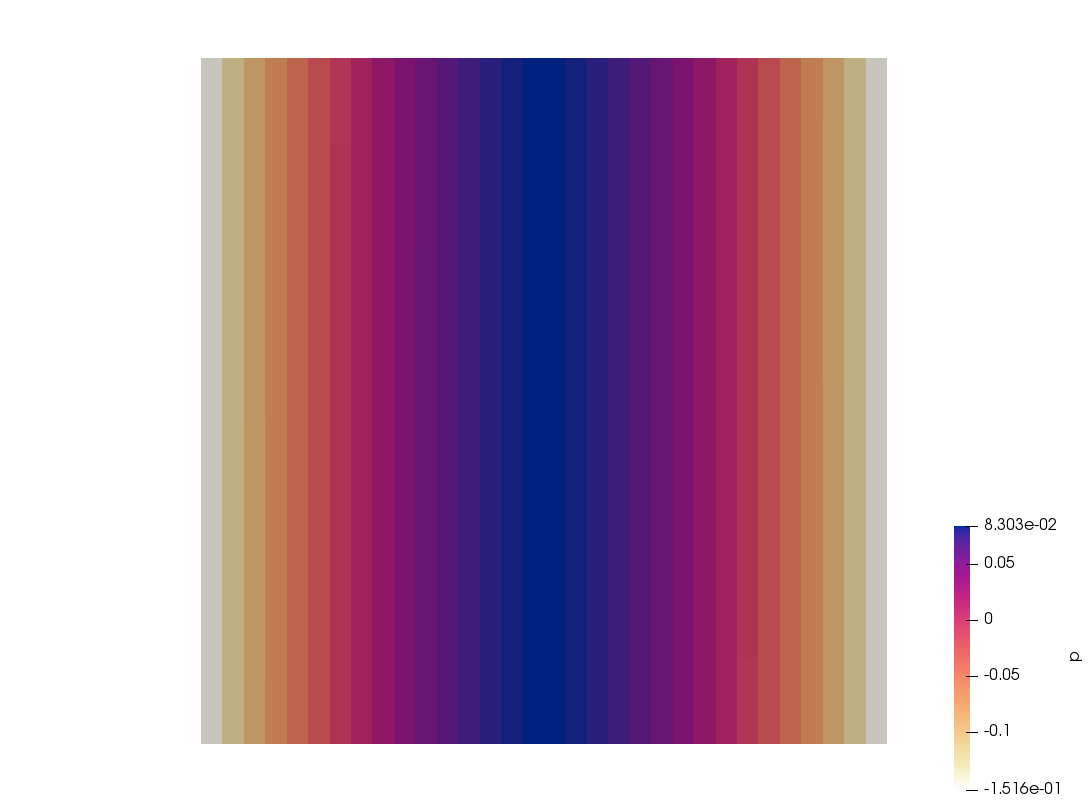
\includegraphics[width=4cm]{python_codes/fieldstone_12/results/reg/p32}
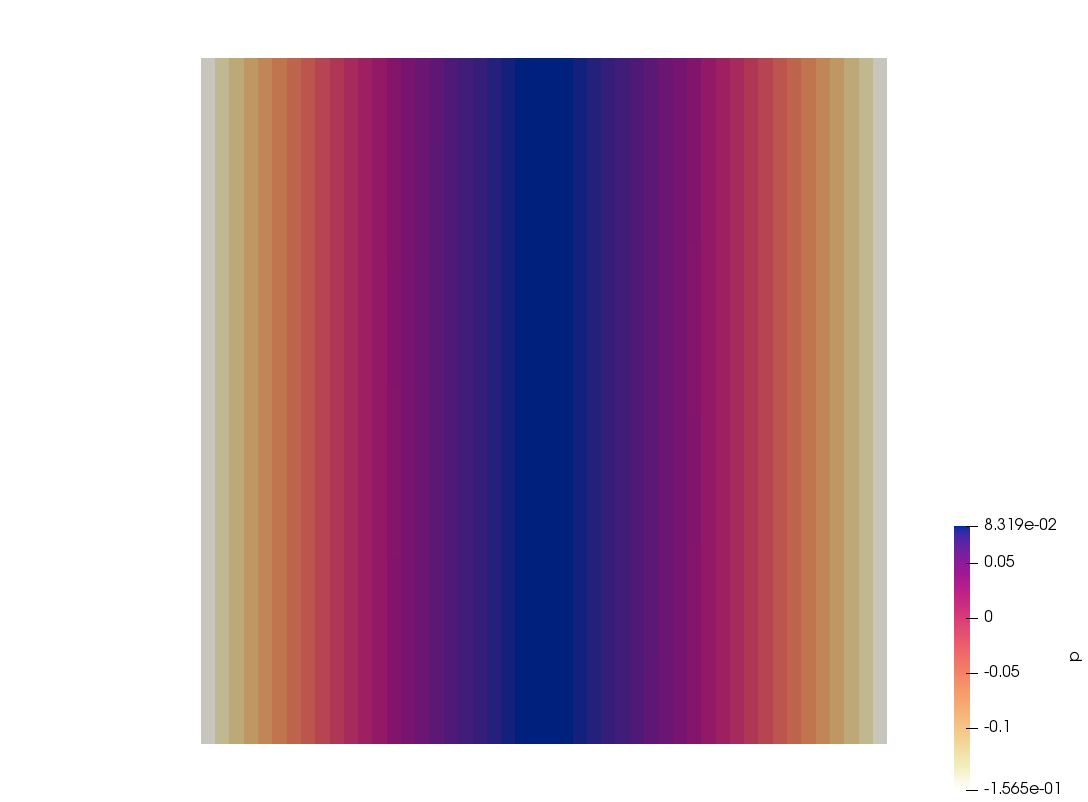
\includegraphics[width=4cm]{python_codes/fieldstone_12/results/reg/p48}
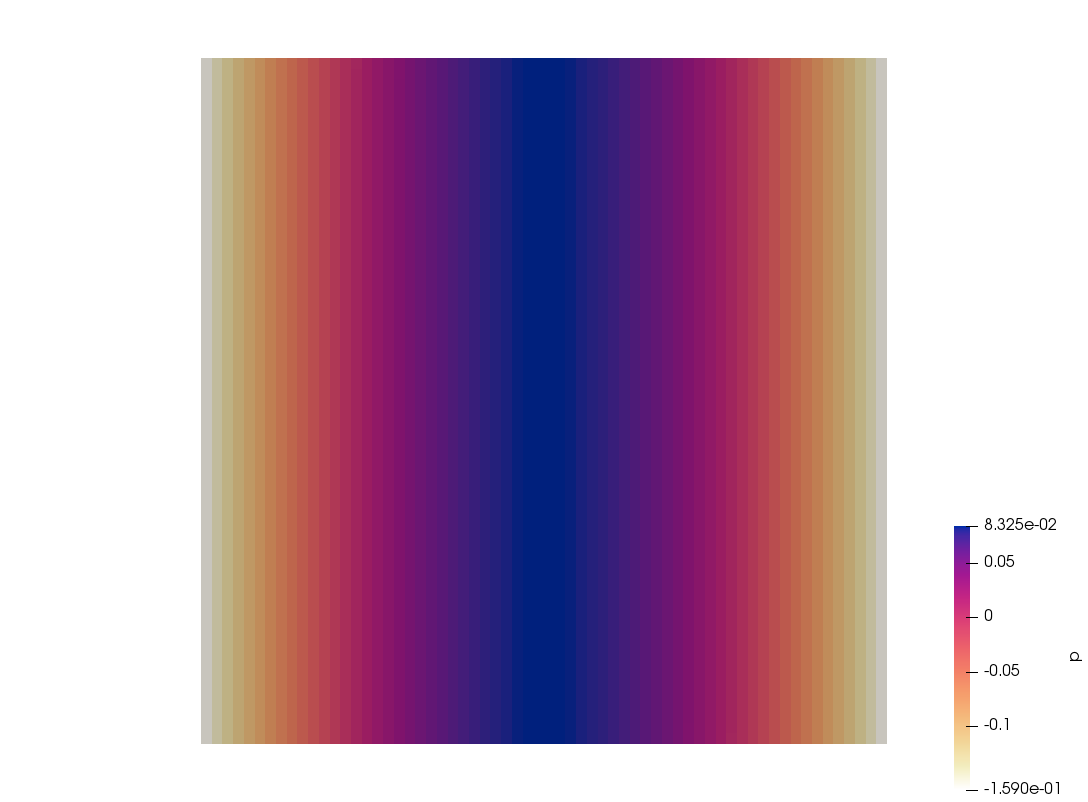
\includegraphics[width=4cm]{python_codes/fieldstone_12/results/reg/p64}\\
{\captionfont Elemental pressure field for 32x32, 48x48 and 64x64 resolutions.}
\end{center}
This means that the algorithms above fulfill an interpolation function, but not a smoothing one.

\newpage
%............................................
\paragraph{Adding randomness to internal node positions} We now add a random value $\xi h$ to the 
location of all nodes which are not on the boundary where $h$=$L_x$/nelx and we set $\xi=20\%$.
In this case a 32x32 mesh looks as follows:

\begin{center}
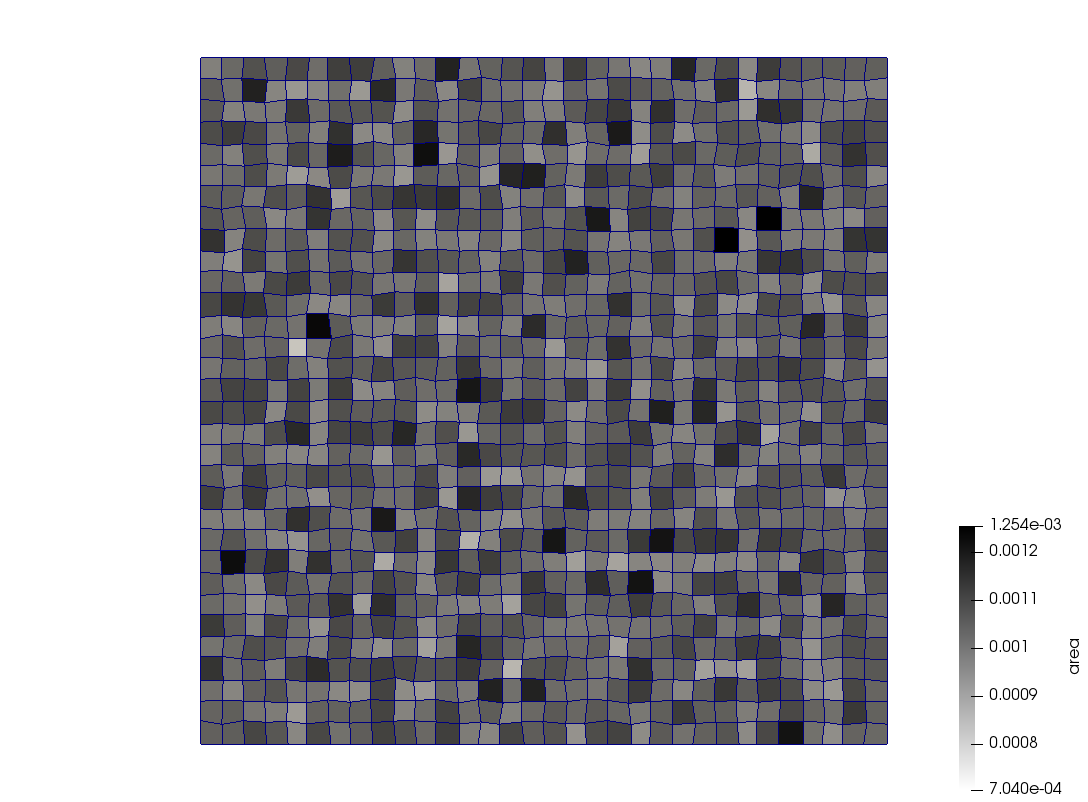
\includegraphics[width=7cm]{python_codes/fieldstone_12/results/rand/area_0p1}
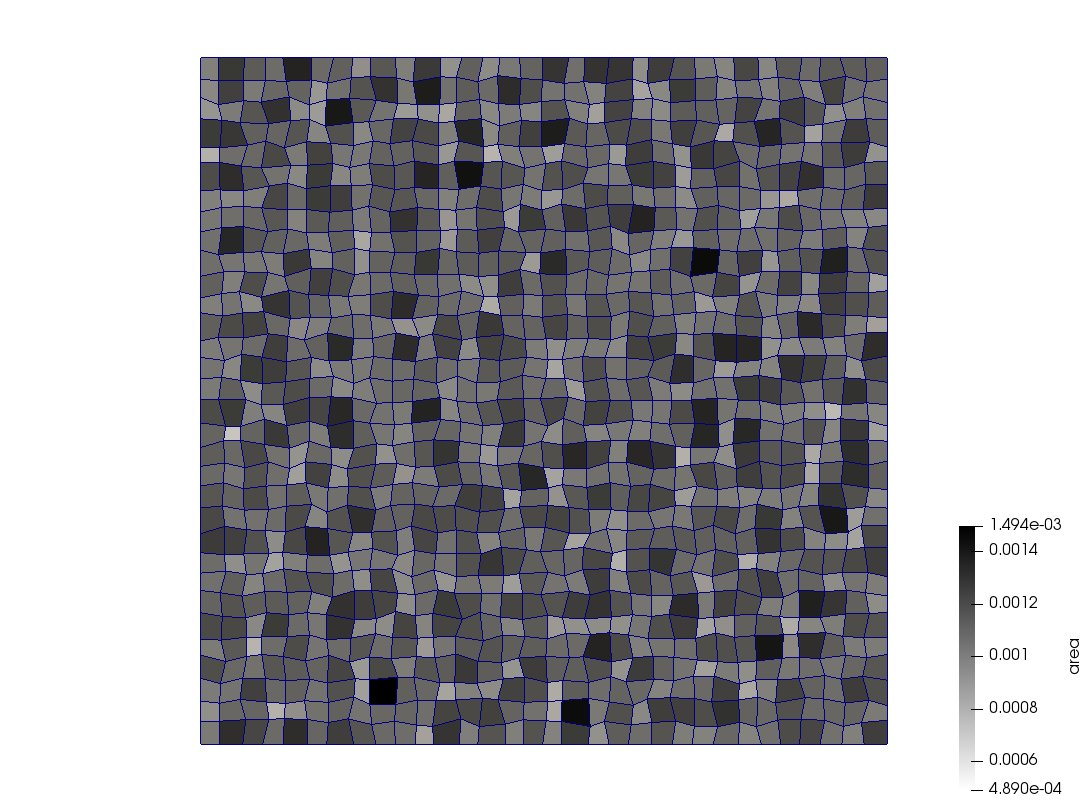
\includegraphics[width=7cm]{python_codes/fieldstone_12/results/rand/area_0p2}\\
{\captionfont Mesh 32x32 elements. Left: $\xi=0.1$; Right: $\xi=0.2$}
\end{center}

We repeat the same exercise as before on such a mesh and look at the errors

\begin{center}
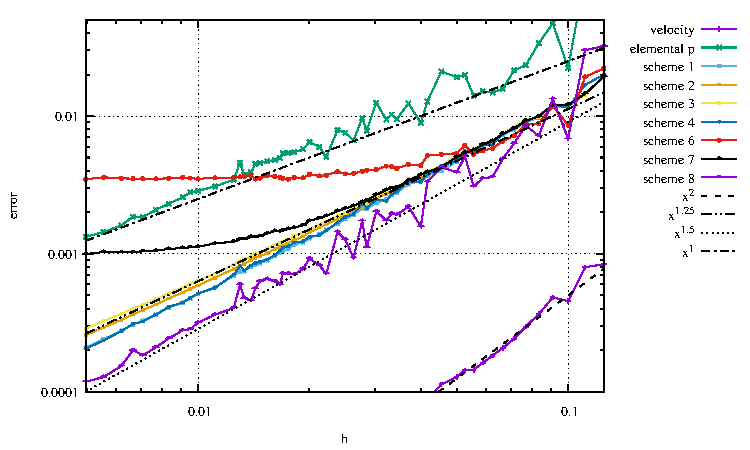
\includegraphics[width=7cm]{python_codes/fieldstone_12/results/rand/errors_nofilter}
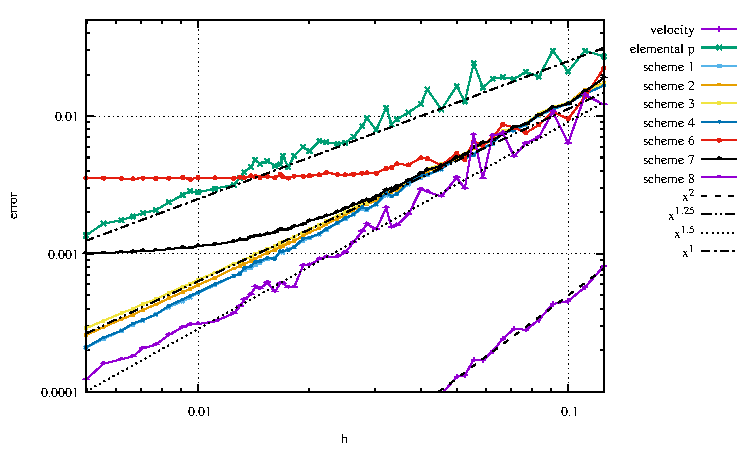
\includegraphics[width=7cm]{python_codes/fieldstone_12/results/rand/errors_filter}\\
{\captionfont Velocity and pressure errors for $\xi=0.2$. Left: no filter, right: with filter.} 
\end{center}

It is easy to see the drastic effect that the filter has on the min/max of the elemental pressure:
\begin{center}
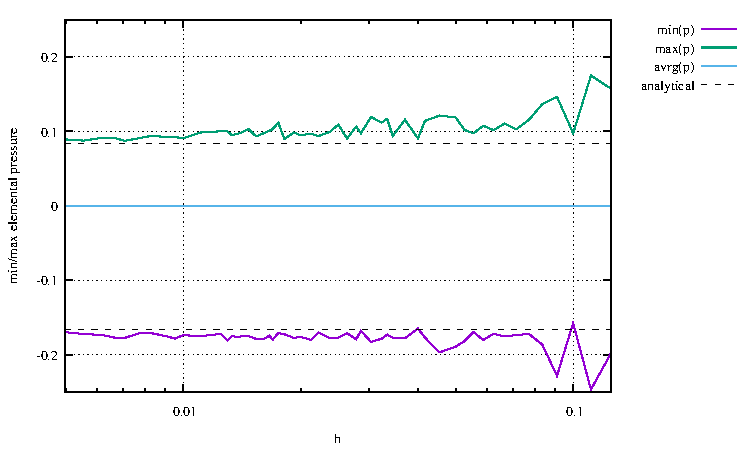
\includegraphics[width=7cm]{python_codes/fieldstone_12/results/rand/rawp_nofilter}
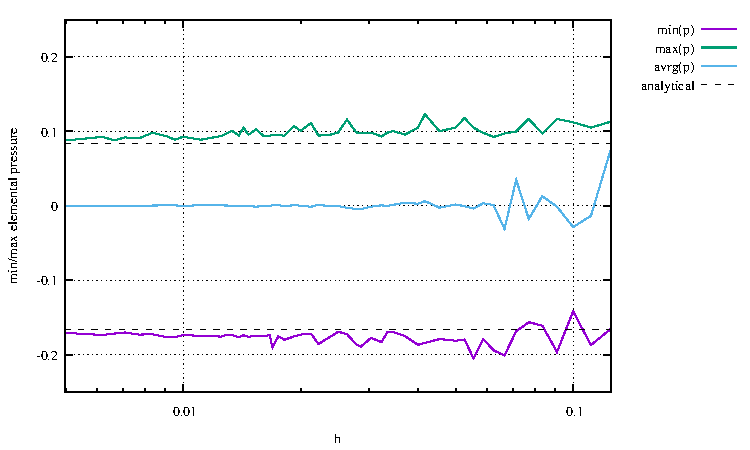
\includegraphics[width=7cm]{python_codes/fieldstone_12/results/rand/rawp_filter}\\
{\captionfont min/max value of elemental pressure field: Left: no filter, right: with filter}
\end{center}

Rather surprisingly we find that $q_1$ still proves to be the most accurate of all pressures and it converges
with $h^{1.5}$(?) as before. Because checkerboard modes are triggered the convergence of the elemental 
pressure is more chaotic but on average linear. 
The $q_6$ and $q_7$ fields seem to unexpectedly stop converging above a given resolution, which 
probably comes from the lack of adequate treatment of sides and corners.
All others converge with $h^{1.5}$ and $q_4$ seems a bit more chaotic than the others.
Scheme 8 seems to be the best here again but with an erratic convergence about $h^{1.5}$

\begin{center}
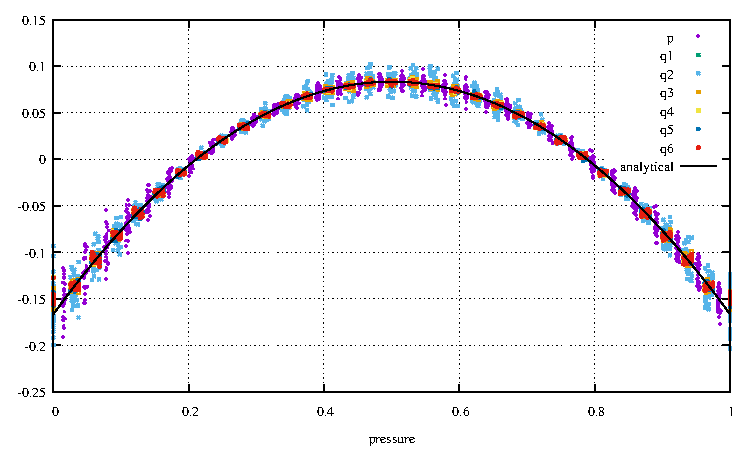
\includegraphics[width=5cm]{python_codes/fieldstone_12/results/rand/pressure}
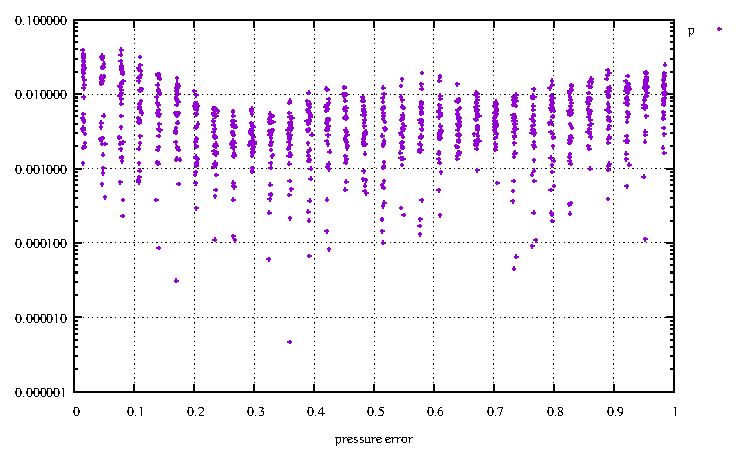
\includegraphics[width=5cm]{python_codes/fieldstone_12/results/rand/p_error}
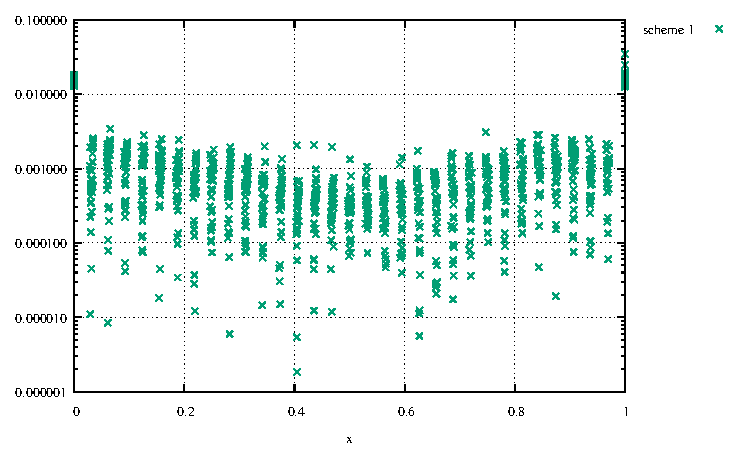
\includegraphics[width=5cm]{python_codes/fieldstone_12/results/rand/q1_error}\\
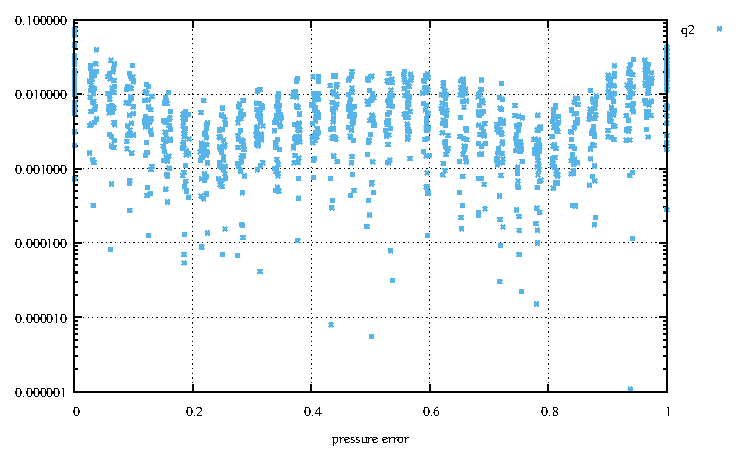
\includegraphics[width=5cm]{python_codes/fieldstone_12/results/rand/q2_error}
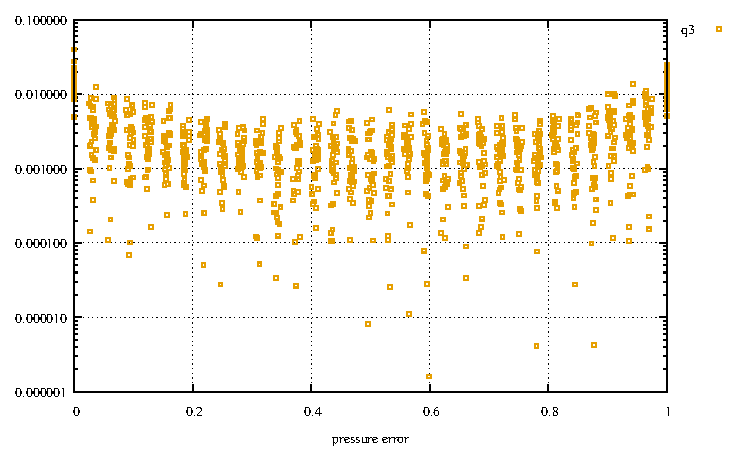
\includegraphics[width=5cm]{python_codes/fieldstone_12/results/rand/q3_error}
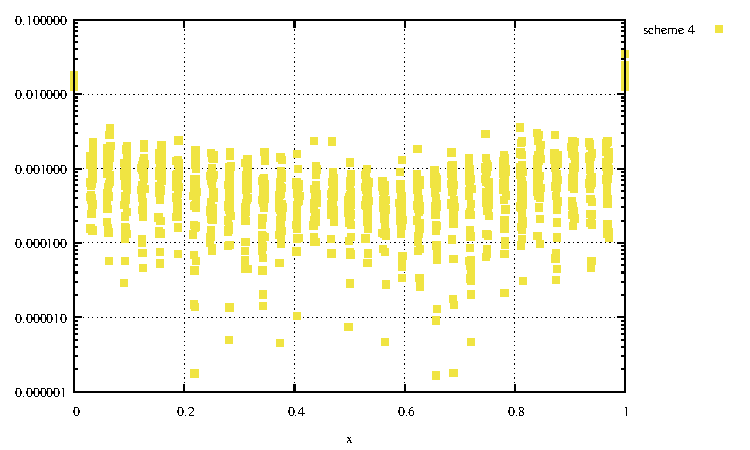
\includegraphics[width=5cm]{python_codes/fieldstone_12/results/rand/q4_error}\\
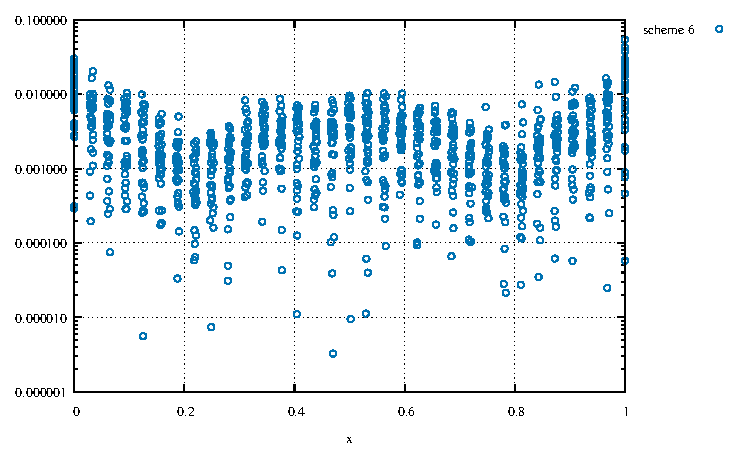
\includegraphics[width=5cm]{python_codes/fieldstone_12/results/rand/q6_error}
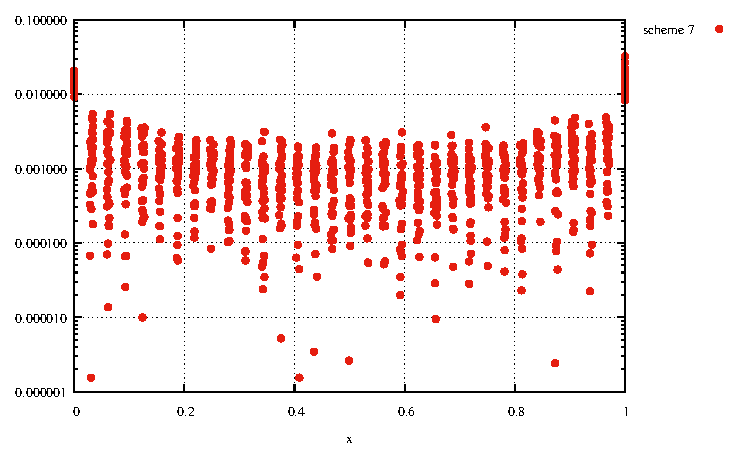
\includegraphics[width=5cm]{python_codes/fieldstone_12/results/rand/q7_error}
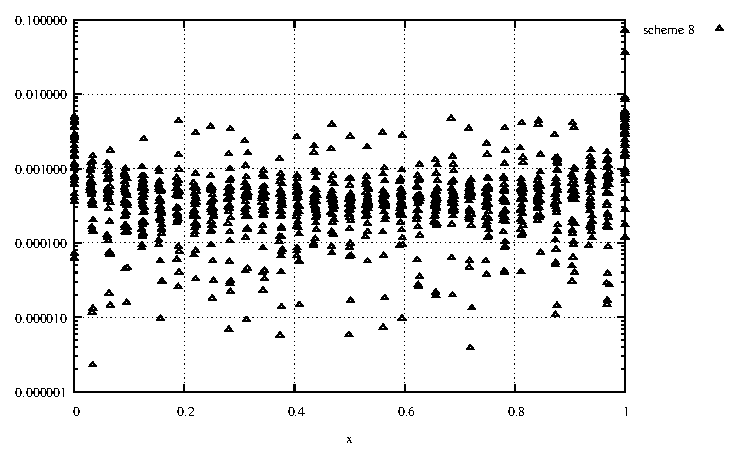
\includegraphics[width=5cm]{python_codes/fieldstone_12/results/rand/q8_error}\\
{\captionfont all obtained in 32x32 mesh}
\end{center}

\begin{center}
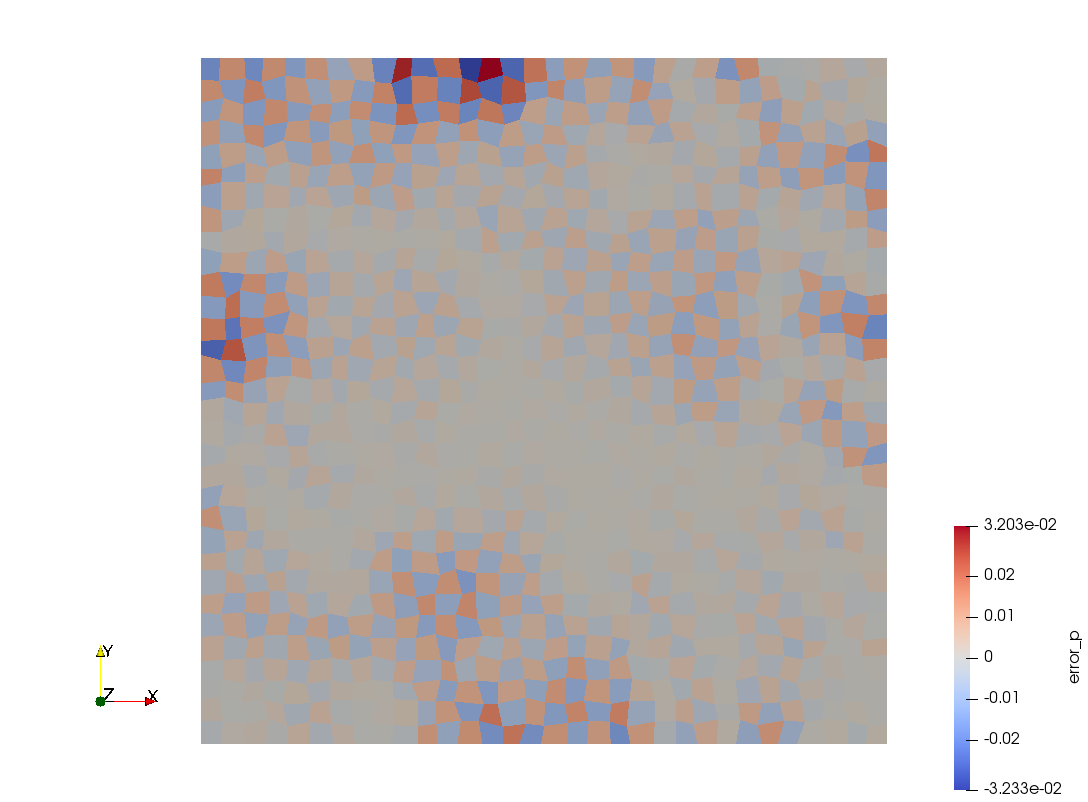
\includegraphics[width=5cm]{python_codes/fieldstone_12/results/rand/errp}
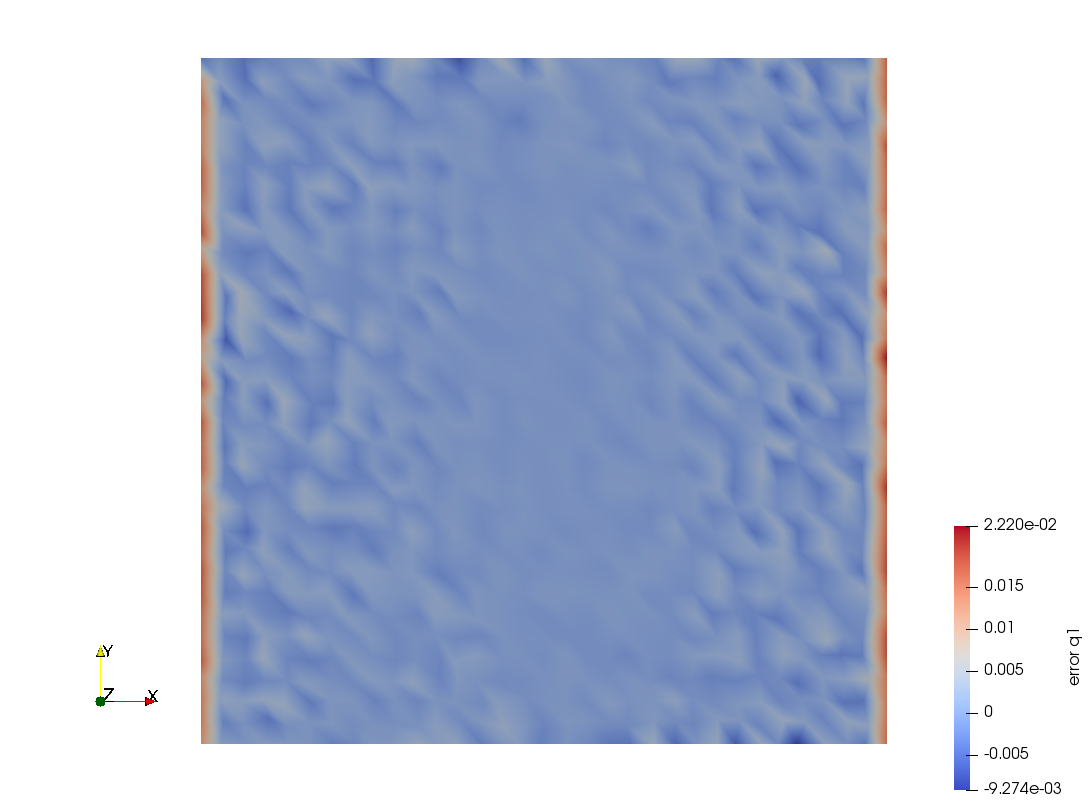
\includegraphics[width=5cm]{python_codes/fieldstone_12/results/rand/errq1}
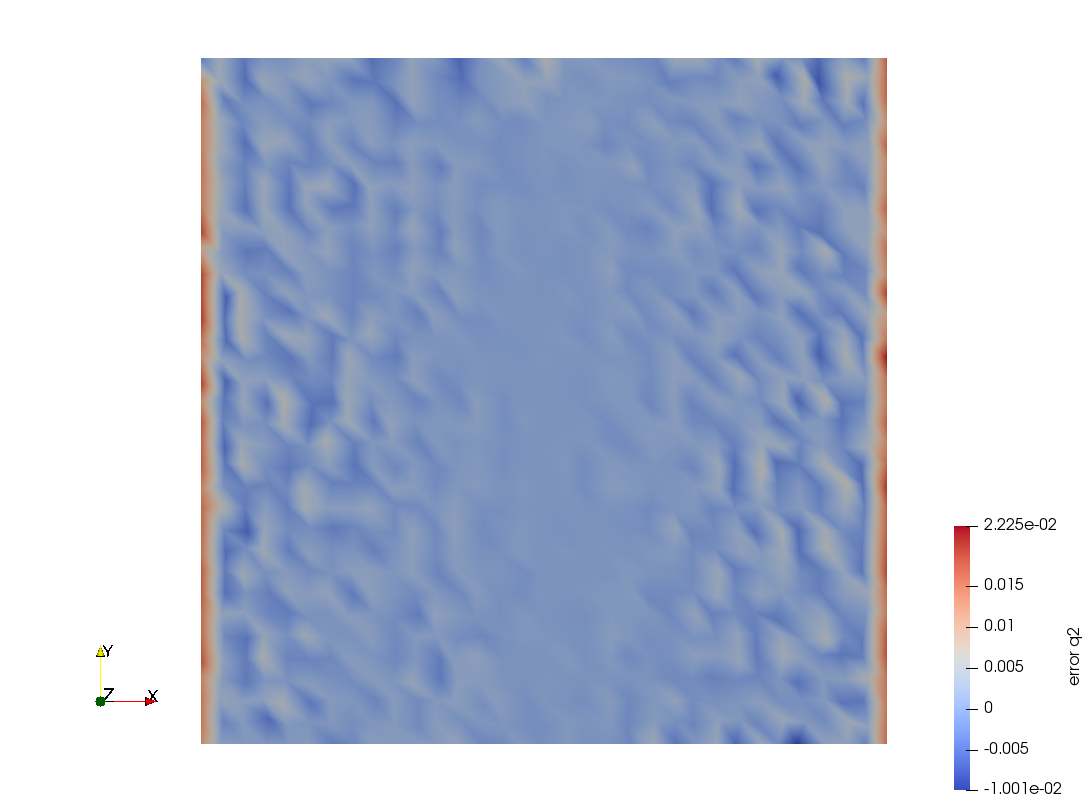
\includegraphics[width=5cm]{python_codes/fieldstone_12/results/rand/errq2}\\
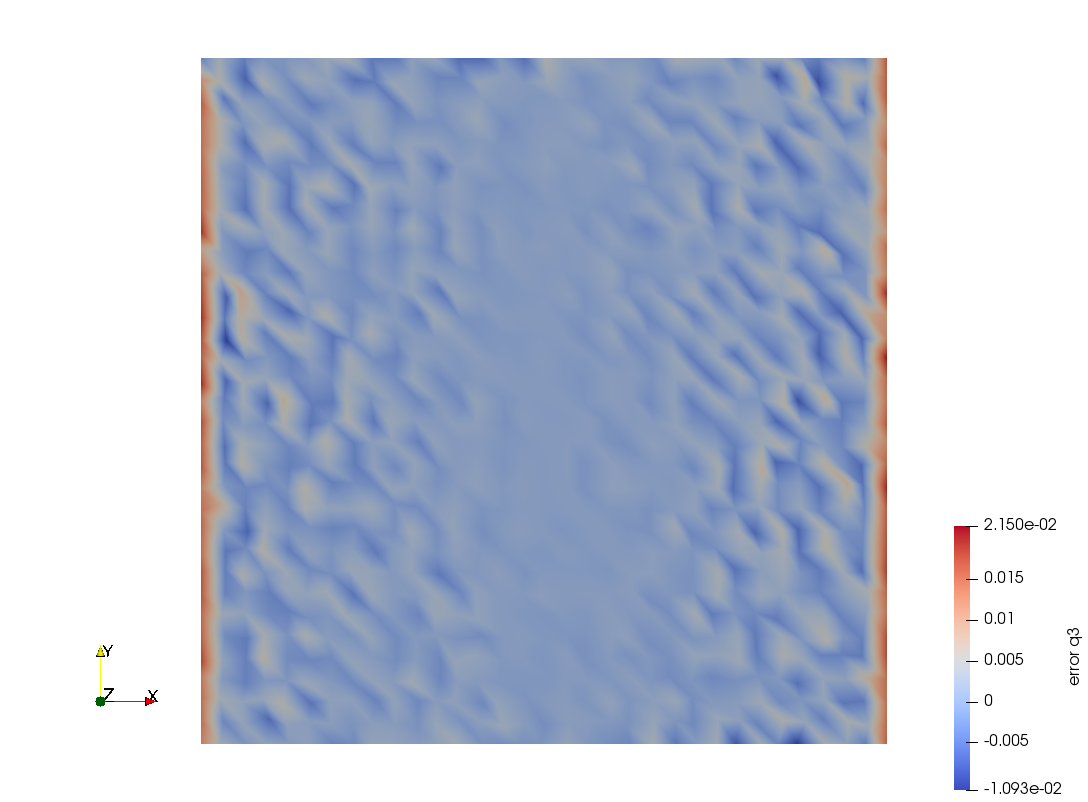
\includegraphics[width=5cm]{python_codes/fieldstone_12/results/rand/errq3}
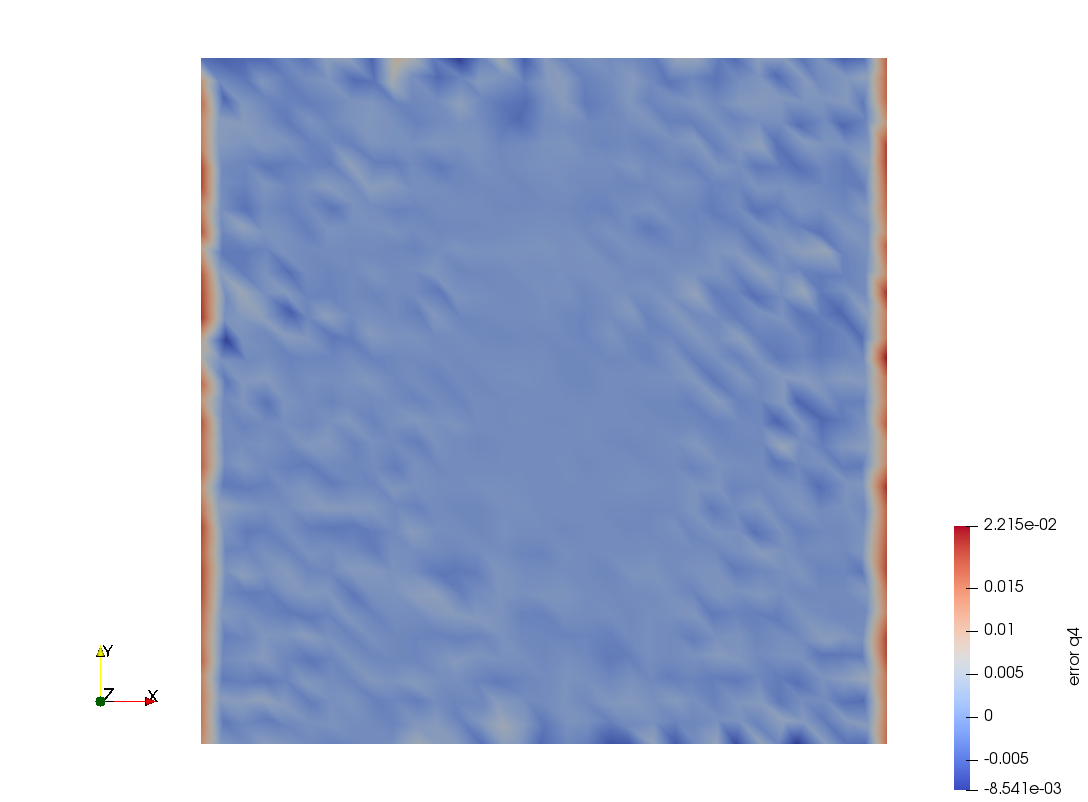
\includegraphics[width=5cm]{python_codes/fieldstone_12/results/rand/errq4}
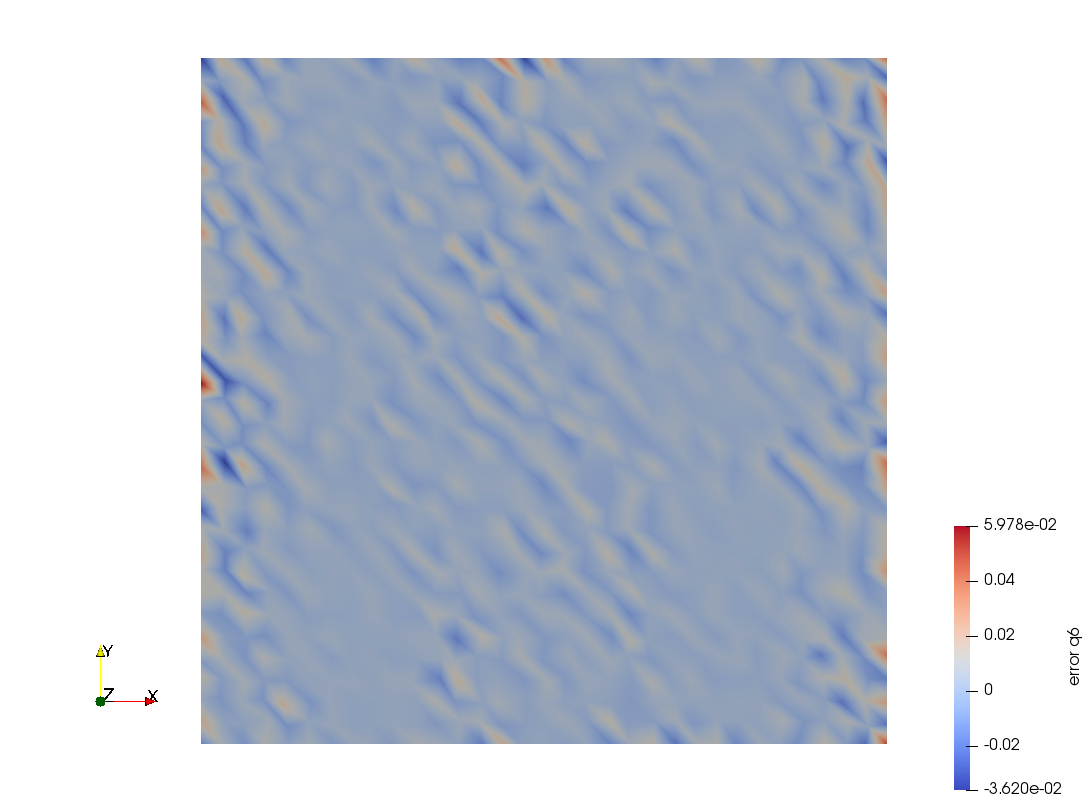
\includegraphics[width=5cm]{python_codes/fieldstone_12/results/rand/errq6}\\
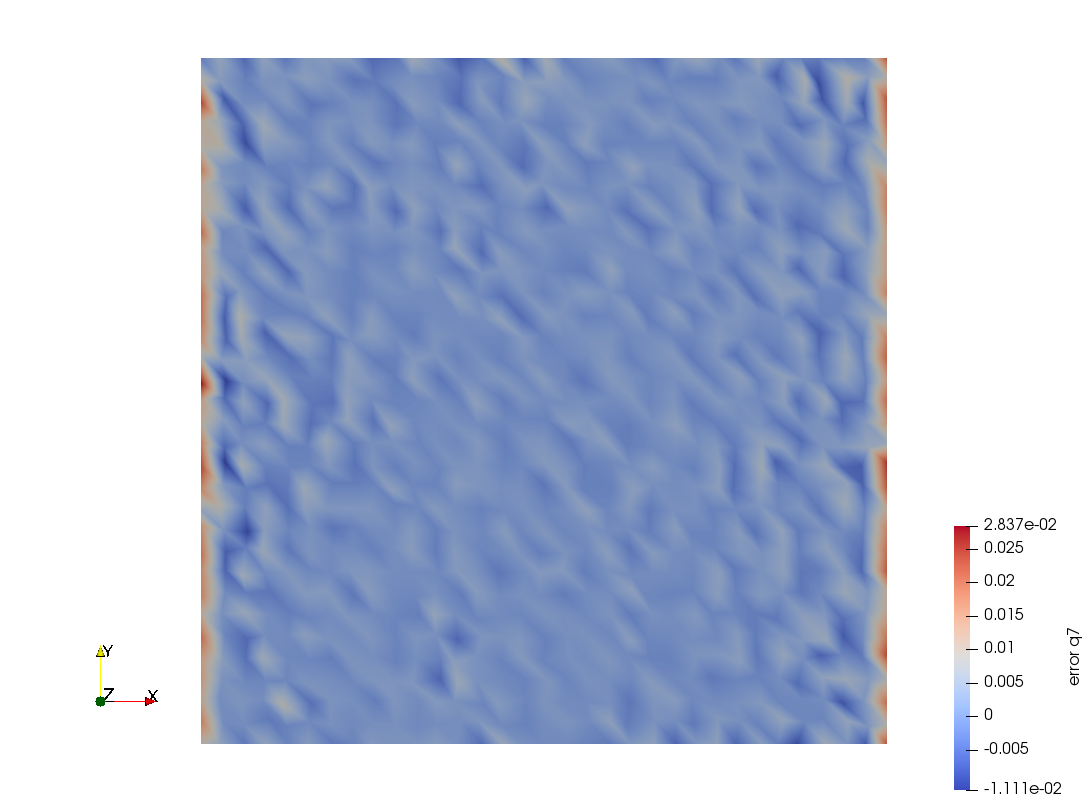
\includegraphics[width=5cm]{python_codes/fieldstone_12/results/rand/errq7}
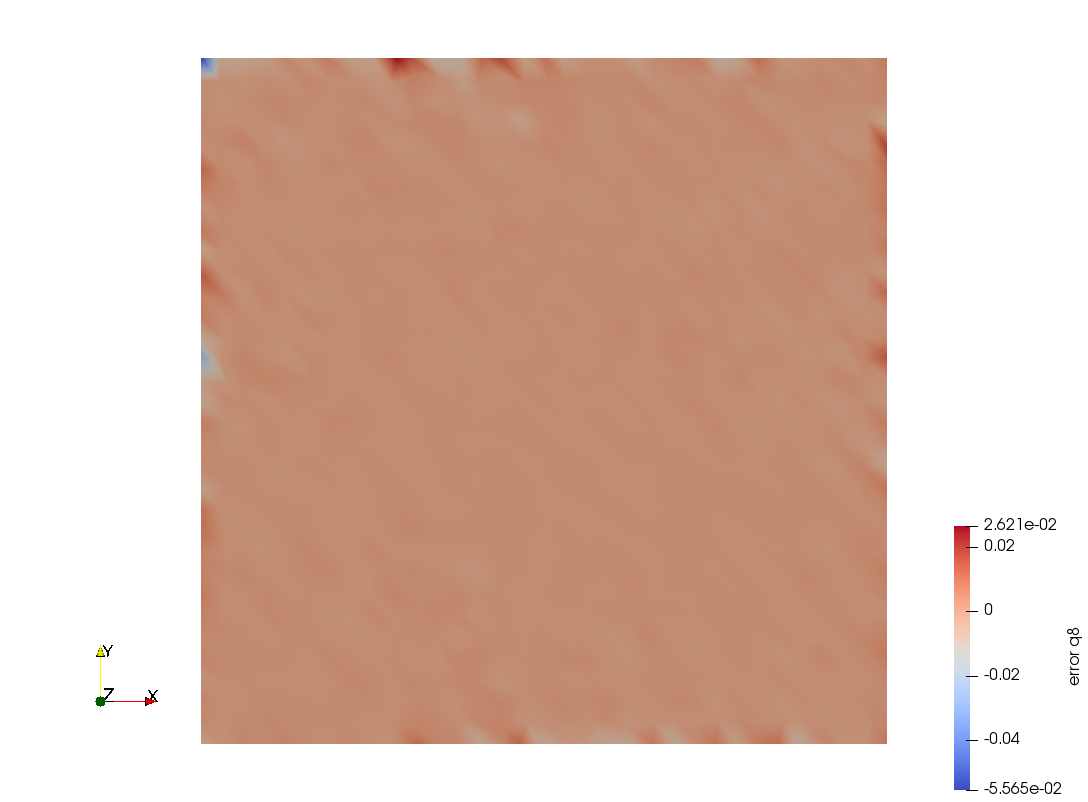
\includegraphics[width=5cm]{python_codes/fieldstone_12/results/rand/errq8}\\
{\captionfont Pressure error for the elemental and nodal pressure fields. Note 
the presence of a spatially varying checkboard pattern in the elemental pressure field.
Obtained on 32x32 mesh.}
\end{center}


\newpage
%............................................
\paragraph{Lid driven cavity}

The domain is a unit square. No slip boundary conditions are prescribed 
on left, right and bottom boundary. Unit velocity is prescribed on the top, 
including both top corners, in order to generate a velocity/pressure discontinuity  
which triggers the checkerboard. This is rather succesful (no filter is applied yet):

\begin{center}
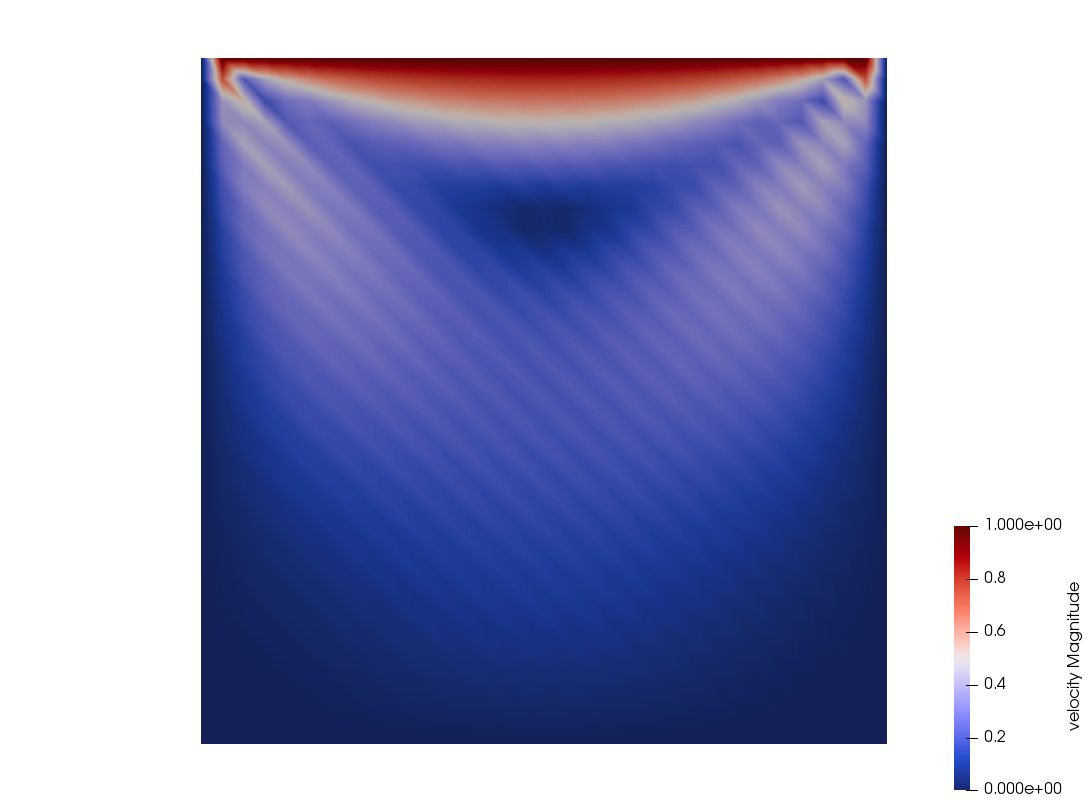
\includegraphics[width=7cm]{python_codes/fieldstone_12/results/ldc32/vel}
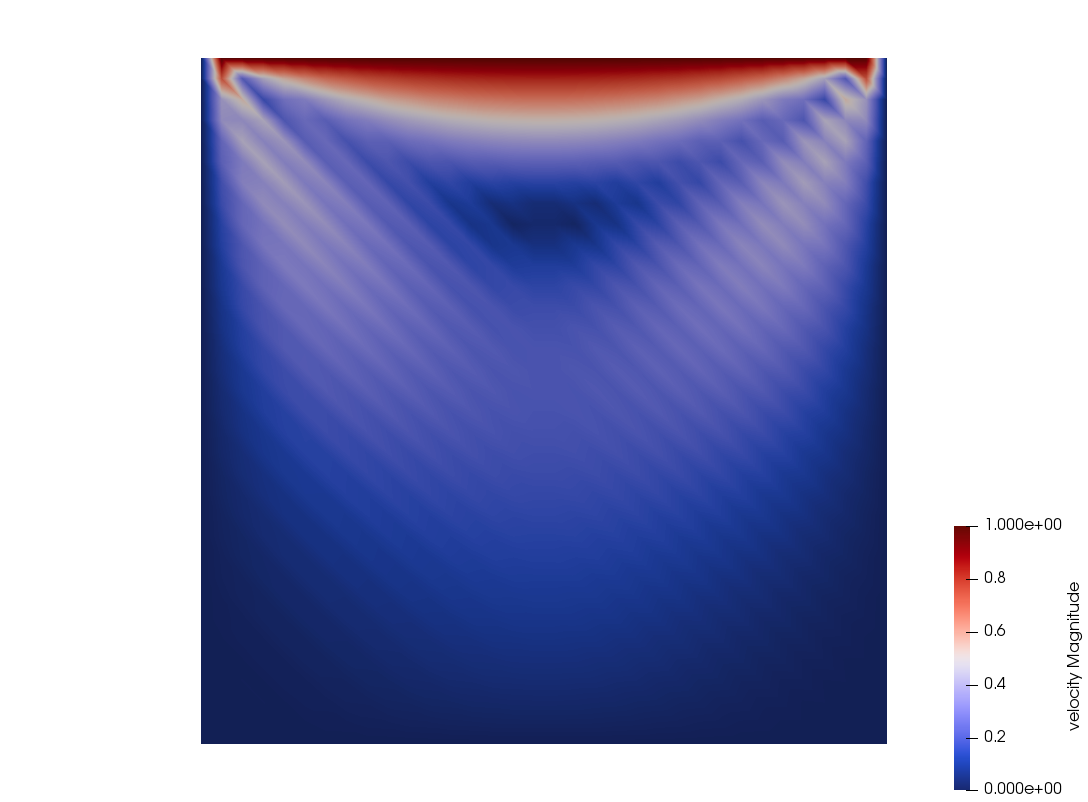
\includegraphics[width=7cm]{python_codes/fieldstone_12/results/ldc33/vel}\\
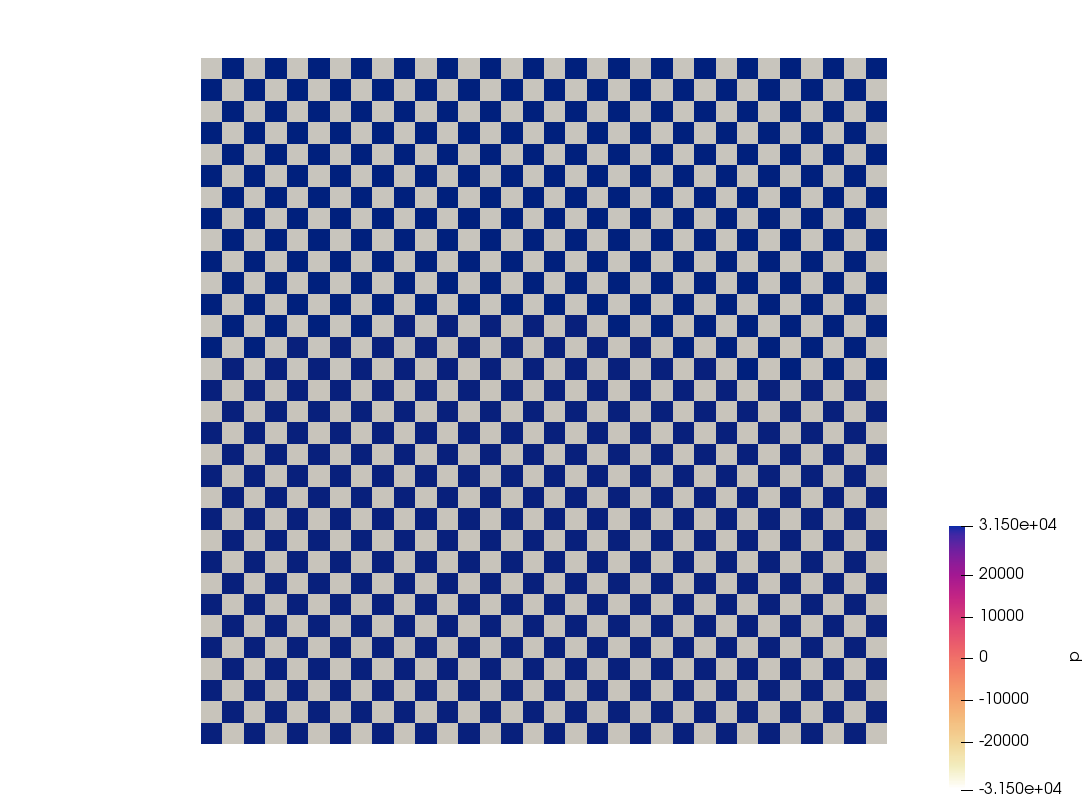
\includegraphics[width=7cm]{python_codes/fieldstone_12/results/ldc32/p}
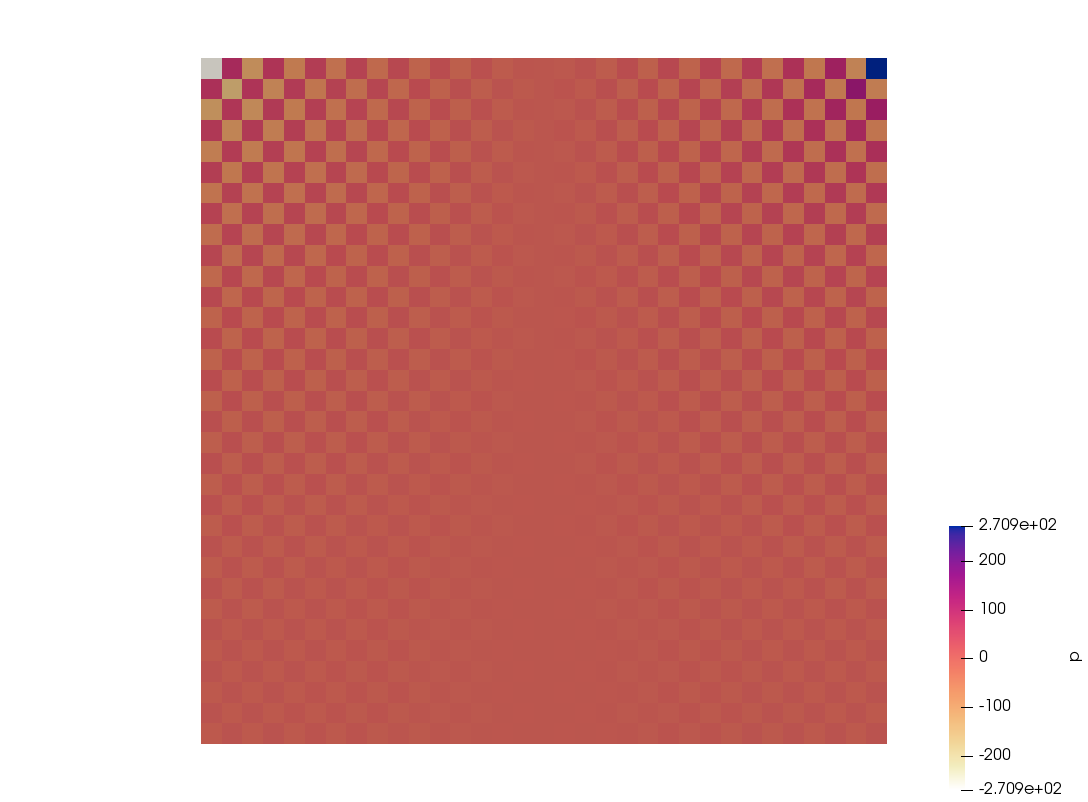
\includegraphics[width=7cm]{python_codes/fieldstone_12/results/ldc33/p}\\
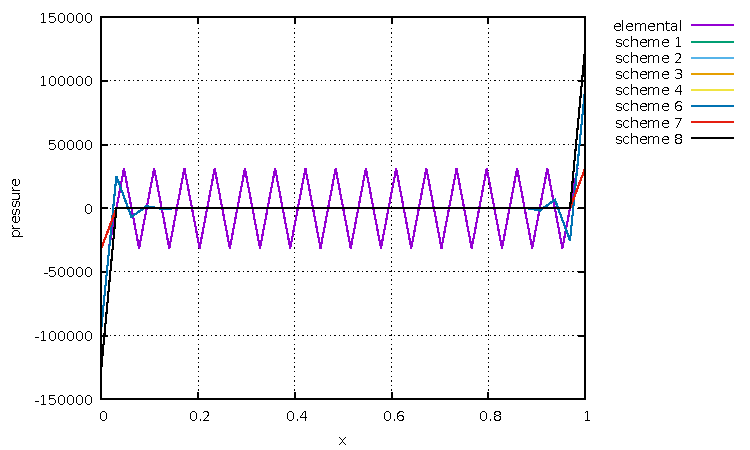
\includegraphics[width=7cm]{python_codes/fieldstone_12/results/ldc32/p_top}
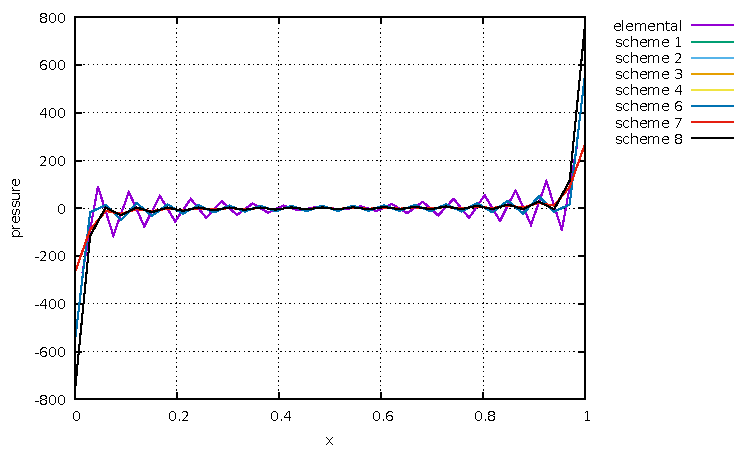
\includegraphics[width=7cm]{python_codes/fieldstone_12/results/ldc33/p_top}\\
{\captionfont Left: 32x32, Right: 33x33. Last row is pressures at the top of the domain.}
\end{center}

We recover the well known fact that even number of elements are more prone to 
checkerboard of high amplitude, but odd numbers do not preclude their presence.
The conclusion is unescapable: there is no nodal pressure filed which does not 
showcase positive/negative oscillations.


It is easy to see the drastic effect that the filter has on the min/max of the elemental pressure:

\begin{center}
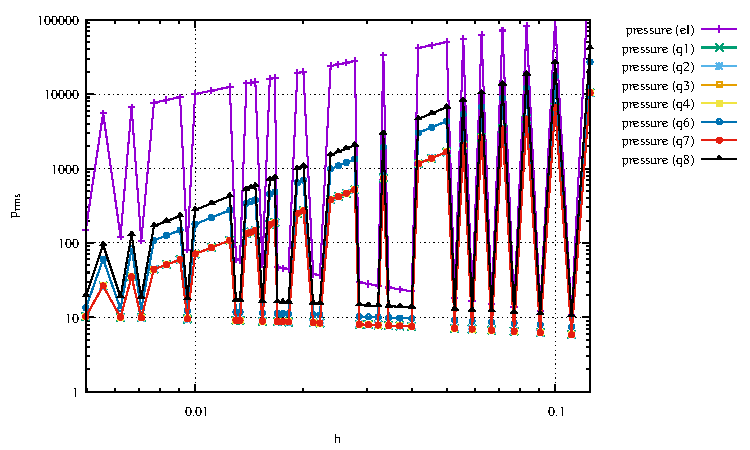
\includegraphics[width=7cm]{python_codes/fieldstone_12/results/ldc/prms_nofilter}
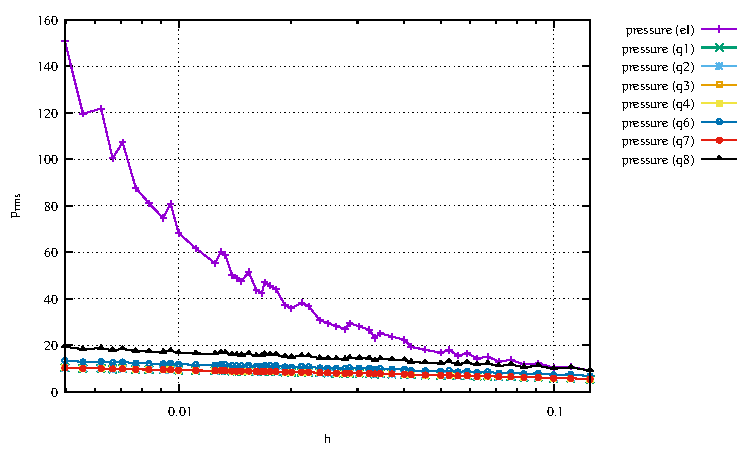
\includegraphics[width=7cm]{python_codes/fieldstone_12/results/ldc/prms_filter}\\
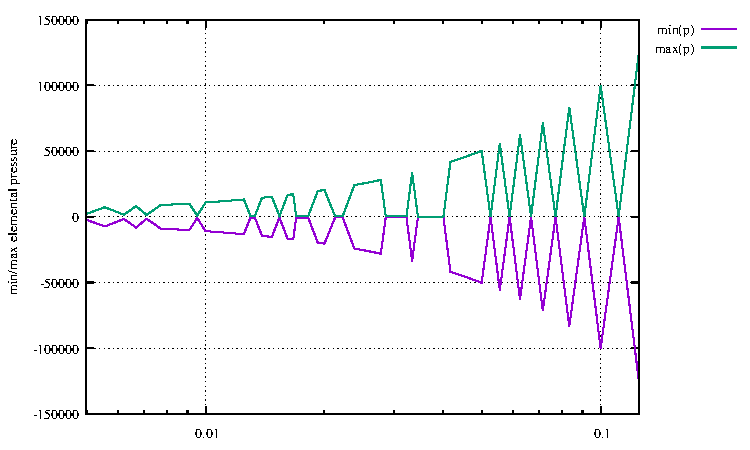
\includegraphics[width=7cm]{python_codes/fieldstone_12/results/ldc/rawp_nofilter}
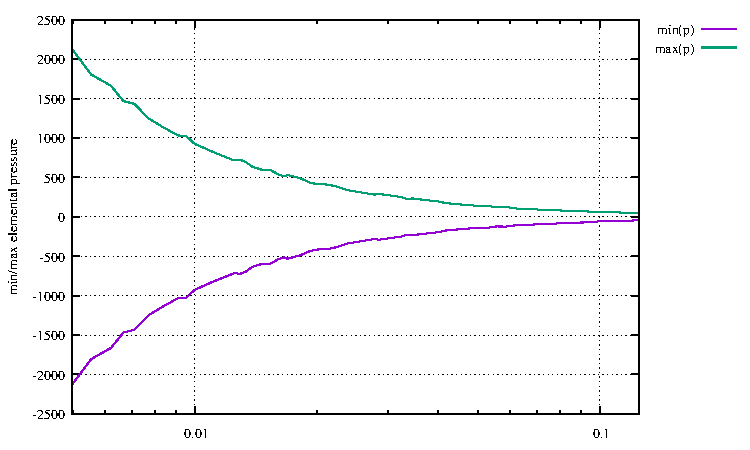
\includegraphics[width=7cm]{python_codes/fieldstone_12/results/ldc/rawp_filter}\\
{\captionfont Left: filter off; Right: filter on}
\end{center}

Only schemes 6 and 7 are unaffected by the filter since they 


%............................................
\paragraph{Regularised Lid driven cavity}

See stone 4. The velocity on the top is given by $u(x)=x^2(1-x)^2$.
This has the advantage of removing the discontinuity at the corners and 
thereby yielding a problem which has a non-singular solution.
However, wee see that the checkerboard mode is still present:

\begin{center}
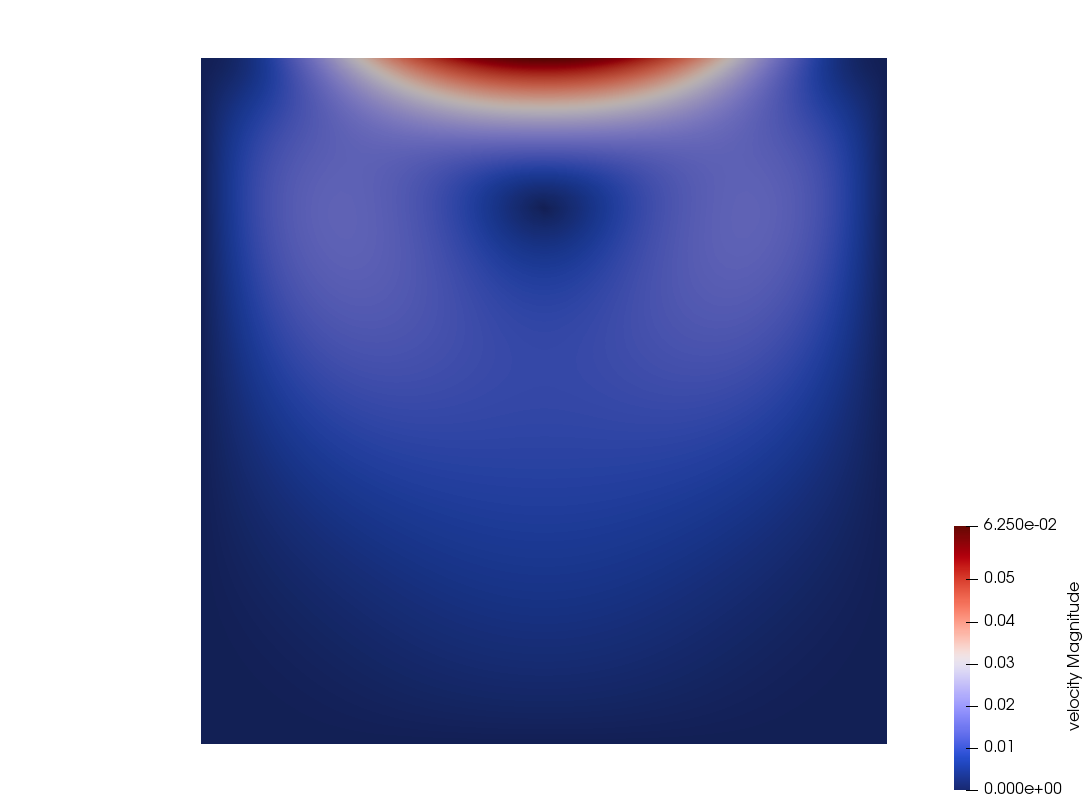
\includegraphics[width=7cm]{python_codes/fieldstone_12/results/rldc/vel}
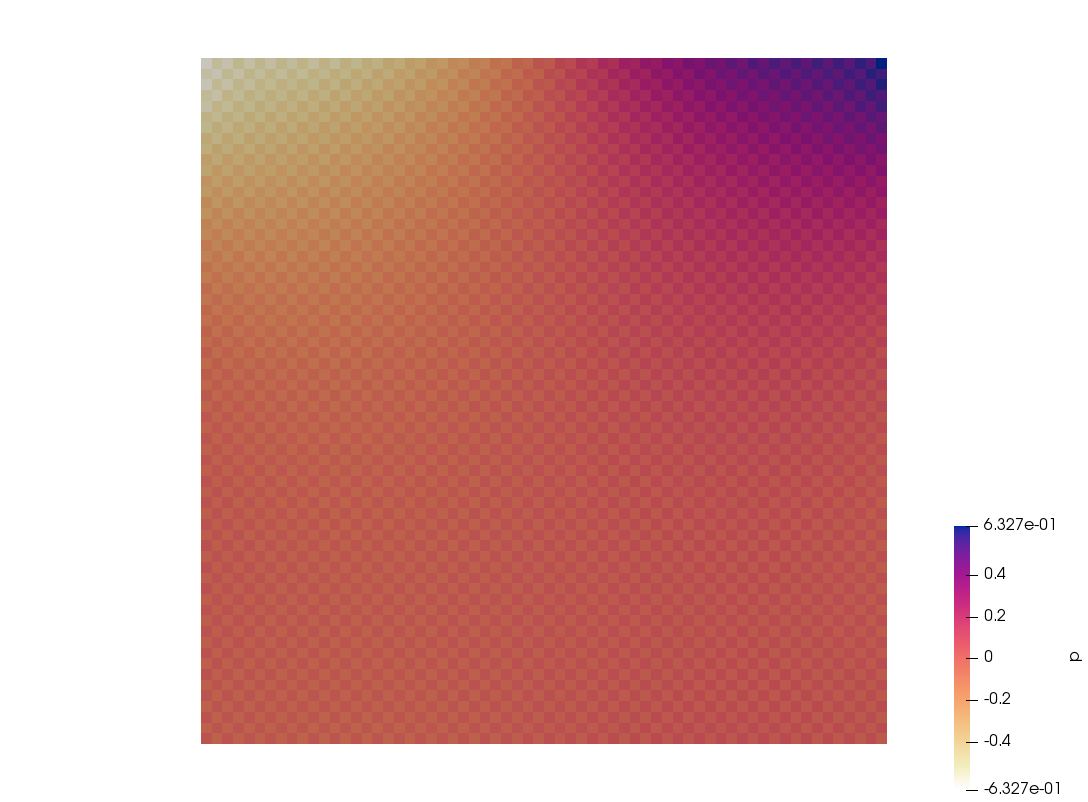
\includegraphics[width=7cm]{python_codes/fieldstone_12/results/rldc/p}\\
{\captionfont Resolution 32x32}
\end{center}

There is no analytical solution. When the pressure errors are computed in the code
the results are actually root mean square pressures (if a zero analytical pressure 
is used). We see that these all converge to a single value.
Here again we see that the filter has a drastic effect on the min/max 
of the elemental pressure. 
\begin{center}
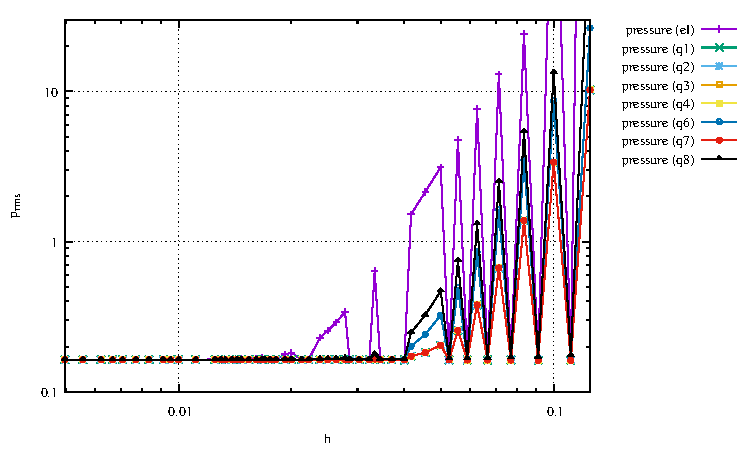
\includegraphics[width=7cm]{python_codes/fieldstone_12/results/rldc/prms_nofilter}
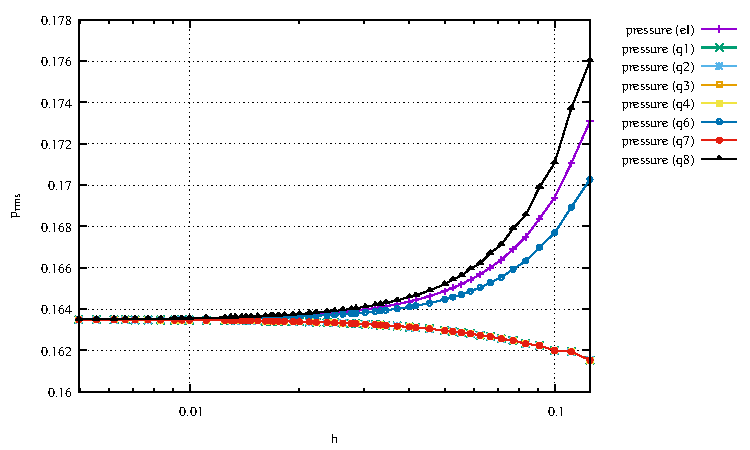
\includegraphics[width=7cm]{python_codes/fieldstone_12/results/rldc/prms_filter}\\
\includegraphics[width=7cm]{python_codes/fieldstone_12/results/rldc/rawp_nofilter}
\includegraphics[width=7cm]{python_codes/fieldstone_12/results/rldc/rawp_filter}\\
{\captionfont Left: filter off; Right: filter on}
\end{center}


